\documentclass[12pt]{article}


\usepackage{amsmath}
%\usepackage{amsthm}
\usepackage{amssymb}

\usepackage[nottoc]{tocbibind}
\usepackage[usenames,dvipsnames,svgnames,table]{xcolor}
\usepackage[colorlinks,citecolor=DarkGreen,linkcolor=FireBrick,urlcolor=FireBrick,linktocpage]{hyperref}
\numberwithin{equation}{section}
\urlstyle{rm}
\def\arxivfont{\rm}
\def\doihref#1#2{\href{#1}{{\color{FireBrick!80!Black}#2}}}
\usepackage{graphicx}
%\usepackage{showkeys}
\usepackage{float}
\usepackage[height=8.8in,width=6.45in]{geometry}
\usepackage{tgtermes}
\usepackage{tgadventor}
\usepackage[scaled]{couriers}
\usepackage[T1]{fontenc}
\usepackage[mathscr]{euscript}
\usepackage[export]{adjustbox}
\usepackage{braket}
\usepackage[safe]{tipa}

\usepackage{xcolor}
\usepackage{mdframed}
\usepackage[amsmath]{ntheorem}
%\theorembodyfont{\normalfont}

\newmdtheoremenv[backgroundcolor=black!10,linecolor=black!0]{definition}{Definition}[section]
\newmdtheoremenv[backgroundcolor=black!10,linecolor=black!0]{theorem}[definition]{Theorem}
\newmdtheoremenv[backgroundcolor=black!3,linecolor=black!0]{example}[definition]{Example}
\newmdtheoremenv[backgroundcolor=black!3,linecolor=black!0]{proposition}[definition]{Proposition}
\newmdtheoremenv[backgroundcolor=black!3,linecolor=black!0]{notation}[definition]{Notation}
\newmdtheoremenv[backgroundcolor=black!3,linecolor=black!0]{fact}[definition]{Fact}
\newmdtheoremenv[backgroundcolor=black!0]{exercise}[definition]{Exercise}



\newenvironment{claim}{  \begin{mdframed}[linecolor=black!0,backgroundcolor=black!10]\noindent\ignorespaces}{\end{mdframed}}

\let\originalfigure=\figure
\let\endoriginalfigure=\endfigure

\renewenvironment{figure}[1][]{
  \begin{originalfigure}[#1]
    \begin{mdframed}[linecolor=black!0,backgroundcolor=black!1]
}{
    \end{mdframed}
  \end{originalfigure}
}


\let\originaltable=\table
\let\endoriginaltable=\endtable

\renewenvironment{table}[1][]{
  \begin{originaltable}[#1]
    \begin{mdframed}[linecolor=black!0,backgroundcolor=black!1]
}{
    \end{mdframed}
  \end{originaltable}
}


\def\baselinestretch{1.04}
% https://tex.stackexchange.com/questions/473627/set-the-short-display-skip-as-in-coxeter-regular-complex-polytopes-1974
%\makeatletter
%\g@addto@macro\normalsize{%
%  \setlength\abovedisplayshortskip{\glueexpr\abovedisplayskip-\baselineskip}%
%  \setlength\belowdisplayshortskip{\belowdisplayskip}%
%}
%\makeatother

\def\Nequals#1{$\mathcal{N}{=}\,#1$}


\definecolor{shadecolor}{rgb}{0.90,0.90,0.90}


\def\important#1#2{%
\begin{mdframed}[linecolor=black!0,backgroundcolor=black!5]
\textbf{#1.} #2
\end{mdframed}
}



\newenvironment{comment}{\par\noindent [Comment. \ }{\par\noindent End comment.]}

\def\inc#1{\vcenter{\hbox{\includegraphics[scale=.2]{#1}}}}
\def\incc#1{\vcenter{\hbox{\includegraphics[scale=.6]{#1}}}}

\def\TODO#1{{\color{FireBrick} #1}}

\usepackage[whole]{bxcjkjatype} 

\definecolor{identifiercolor}{rgb}{.4,.6,.56}
\definecolor{stringcolor}{gray}{0.5}
\definecolor{inactivecolor}{rgb}{0.15,0.15,0.5}

%%list alg-top-notes

\def\bC{\mathbb{C}}
\def\bH{\mathbb{H}}
\def\bK{\mathbb{K}}
\def\bR{\mathbb{R}}
\def\bZ{\mathbb{Z}}

\def\cH{\mathcal{H}}

\def\sT{\mathsf{T}}

\let\bar\overline

\def\RP{\mathbb{RP}}
\def\CP{\mathbb{CP}}
\def\HP{\mathbb{HP}}
\def\KP{\mathbb{KP}}

\begin{document}

\centerline{\Large Algebraic topology for physicists}

\bigskip

\centerline{\large Yuji Tachikawa}

\setcounter{tocdepth}{2}
\tableofcontents

\newpage



\section*{Acknowledgements and a disclaimer}

I'd like to thank our Physics Department for giving me this opportunity to give this course.
I'd like to ask participants to point out as many errors as possible in these notes and also during lectures.

This is the first time I'm heavily utilizing AI to prepare my lecture notes.
More concretely I'm using GitHub Co-pilot for \LaTeX, which is based on Chat-GPT.
This tool suggests sentences or paragraphs while writing the notes;
the suggestions are not always perfectly correct, but they are often useful,
with mostly correct \LaTeX\ macros.
But I fear that in some sense I'm plagiarizing the contents used to train the AI.
At least for these notes, I don't think it is particularly problematic,
since the contents of this course are mostly well-known and not my original work.
The possibly only original part is the selection of the contents and the order of presentation.\footnote{%
But this particular sentence was also auto-suggested by Co-pilot, when I typed `The possibly only'...
}
If anybody notices any parts which look like a direct copy from some other source, please let me know.

\section{General introduction}

\subsection{Why now?}
\label{sec:whynow}

Even though there are a number of mathematical physicists in our physics department,
there has been no course on mathematical physics in the graduate school,
at least since when I got hired about ten years ago.
I always wanted to give one such course, but I know 
there are a lot of bureaucratic hurdles to be cleared before adding a lecture slot with a new subject name in the curriculum.

Last year, I noticed that there already actually is a lecture slot with the name
数理物理学 (mathematical physics)
which was somehow not used for about 20 years.
It turns out reviving a long dormant lecture slot requires almost no paperwork,
so I decided to do just that.

Mathematical physics can mean many things. 
It is often distinguished from mathematical methods for physicists (which has a distinct translation in Japanese, 物理数学).
It often means those parts of theoretical physics where the discussions are mathematically rigorous,
e.g.~the part of statistical physics where the existence of thermodynamic limit or of phase transitions are rigorously proved.
It can also mean those parts of theoretical physics where various mathematical concepts are heavily used, albeit not quite rigorously,
such as string theory.


I'm not sure how other faculty member would use this slot in the future,
but my goal this year is to provide an introduction to algebraic topology for physicists,
so it's closer to a course on mathematical methods for physicists,
although the sub-subject of mathematics covered is somewhat different from the usual ones (calculus, linear algebra, a bit of group theory, etc.).
My rationale is the following.

As you already know, math plays a very important role in physics, 
as was famously pointed out by Wigner in his essay \cite{WignerUnreasonable}.
But it is definitely \emph{not} that all subfields of math are equally important.
Clearly important ones are:
\begin{itemize}
  \item \textbf{Calculus:} in some sense this subject arose from physics (by Newton etc.)
  \item \textbf{Linear algebra:} this is important for anything which deals with first-order approximations. 
  It is also a crucial ingredient of quantum mechanics (QM).
  \item \textbf{Theory of Hilbert spaces:} equally important for QM.
  \item \textbf{Group theory:} Symmetry is one of the fundamental concepts in physics. It gives rises to conserved charges in both analytical mechanics and quantum mechanics, for example.
  \item \textbf{Differential geometry:} this is important for general relativity (GR).
\end{itemize}

But there are also ones whose usefulness is quite dubious (or at least not immediately obvious):
\begin{itemize}
  \item \textbf{Number theory:} physics is primarily based on $\bR$ and $\bC$, 
  while the number theory is about $\bZ$.
  \item \textbf{Algebraic geometry:} this is about shapes of objects defined by polynomial equations. 
  Why should physicists care about polynomial equations?
  \item \textbf{Mathematical logic / set theory:} Will we ever use G\"odel's incompleteness theorem in physics?
  Will physics depend on the choice of the particular axioms of set theory?
\end{itemize}

\textbf{Algebraic topology} was in the middle of these two lists, until about 15 years ago.
From 1970s, basic homotopy theory was used in the study of topological solitons 
in particle physics and in condensed matter physics.
Starting in the 1980s, 
some characteristic classes were used in the study of anomalies in particle physics
and in the study of quantum Hall effects in condensed matter physics.
But that was about it.
The algebraic topology used was also quite elementary from mathematician's perspective:
everything used on the physics side was developed 1940s, say.
So  algebraic topology is not usually (and does not have to be) covered in a typical physics curriculum,
or textbooks on mathematical methods for physicists.

But that changed in the last 15 years. 
Topological insulators and superconductors became a hot topic,
and soon we learned that they are classified by K and KO theory \cite{Schnyder:2008tya,Kitaev:2009mg,Ryu:2010zza}.
And they are classification of non-interacting phases.
The study of interacting phases, of a class often known as \emph{symmetry protected topological (SPT) phases},
or as \emph{invertible phases}, 
pursued e.g.~in \cite{Fidkowski:2009dba,Chen:2011pg,Gu:2012ib,Metlitski:2014xqa} 
soon gave rise to the realization that the classification would be done by bordism groups \cite{Kapustin:2014dxa}
or by more general cohomology theories \cite{KitaevCollapse}.
This expectation was confirmed later by \cite{Freed:2016rqq,Yonekura:2018ufj},
where it was shown that the classification of the SPT phases is done by 
the Anderson (or Pontryagin) dual of the bordism group.
This also implicitly gave a general theory of anomalies on the particle physics side.
To understand all this requires a far more advanced algebraic topology than was necessary before
(although still not very modern from mathematicians' point of view, 
since it only uses algebraic topology up to 1970 or something).

To understand this fascinating development required me to learn bits and pieces of algebraic topology 
from various sources. But there is no single place where most of the relevant materials for physicists
are gathered. 
This set of lectures is my attempt to provide such a place.

\subsection{What is algebraic topology? Is it any good?}

Topology is a subfield of math where people study spaces.
Spaces of course appear in physics. 
The four-dimensional spacetime we live in and study via general relativity is a mathematical space.
The space of configurations of a rigid body is also a space.
Similarly, the order parameter of a condensed matter system is a space.
The space of all possible gapped condensed-matter Hamiltonians defined on a lattice 
is also a space.
So, methods to study spaces (i.e.~topology) should be useful to us.

In algebraic topology, we study spaces by associating algebraic objects to them.
Given a space $X$, some of the algebraic objects associated are:
\begin{itemize}
\item \textbf{Homotopy groups:} $\pi_n(X)$ is the group obtained by considering maps $S^n \to X$,
where $S^n$ is the $n$-dimensional sphere (in the convention that the ordinary sphere is $S^2$).
\item \textbf{Bordism groups:} $\Omega_n(X)$ is the group obtained by considering maps $M_n \to X$,
where $M_n$ is a general smooth manifold of dimension $n$.
\item \textbf{Homology groups:} $H_n(X)$ is the group obtained by considering $n$-dimensional `cycles' (essentially polyhedra)
 in $X$, where a cycle is a more general notion than spheres or manifolds.
\end{itemize}
Note that the `source spaces' in the descriptions above has the inclusion relation \begin{equation}
  \{\text{spheres}\} \subset \{\text{manifolds}\} \subset \{\text{cycles}\}
\end{equation} and somehow the difficulty of the computation decreases as the source spaces become more general,
so that the homotopy groups are the most difficult to compute and the homology groups are the easiest.

Homotopy groups are useful to describe topological solitons,
and bordism groups play important roles in the study of topological phases
and of anomalies of quantum field theories.
We will also encounter K-theory $K(X)$, whose difficulty of computation and of definition lies between homotopy and homotopy 
and is similar to that of bordism groups, 
which is useful in the study of non-interacting topological phases
and of properties of fermion fields in quantum field theories.
Homology groups are not as directly relevant for physics at this point of our discussion,
but as the easiest to compute, obtaining them is a first step in the computation of other algebraic objects.

Another topic is the study of fiber bundles $E$ over a space $X$.
This is a space $E$ with a projection $E\to X$ such that, locally around each point $x\in X$, 
$E$ looks like $U\times F$ where $x\in U\subset X$ is a neighborhood of $X$ and $F$ is a fixed space called the fiber.
Topology of fiber bundles are often distinguished by the help of characteristic classes,
again a topic of algebraic topology.
This appears in many places in physics. Three examples:
\begin{itemize}
\item Gauge fields (such as the Maxwell field or the Yang-Mills field, describing the electromagnetism or the strong force)
mare mathematically described by connections on fiber bundles, where the base space $X$ is our spacetime.
The topology of this fiber bundle gives rise to Dirac monopoles and instantons,
specified by the characteristic classes known as the 1st and 2nd Chern classes of the bundle, respectively.
\item Consider a crystalline system in a condensed matter setting. The band structure of the system
determines a fiber bundle (of Hilbert spaces) over the Brillouin zone. 
Its topology underlie many of the topological properties of the system.
For example, for a $2+1$ dimensional system, 
the 1st Chern class of this bundle (which is an integer) gives the quantized Hall conductance,
as the famous analysis of Thouless, Kohmoto, Nightingale, and den Nijs showed \cite{Thouless:1982zz}.
\item A parameterized family of quantum states can also be considered as a fiber bundle over the parameter space,
where the fiber can be either the Hilbert space of wavefunctions or the space of density matrices.
The topology of this fiber bundle gives rise to the notion of Berry phase.
We will also see that there are cases such that there can be a continuous family of density matrices
which is never realized as a continuous family of statistical mixture of wavefunctions.
Again this issue is detected by a characteristic class, known as the Dixmier-Douady class.
\end{itemize}
Characteristic classes of fiber bundles often take values in cohomology groups of the base space $X$,
which also explains the usefulness of (co)homology groups in physics.

The aim of this lecture series is to provide a minimal amount of information so that you can understand 
the content of the paragraphs above.
This will, unfortunately, require the whole semester.

\subsection{Mathematical rigor in the course}
This is not a course for (prospective) mathematicians. 
For me, math is like a collection of useful apps (on your Mac/PC or mobile devices).
Here is a comparison chart:
\begin{center}
\begin{tabular}{|c|c|}
  \hline
  math & app \\
  \hline
  definition & short usage of the app \\
  theorem & app itself \\
  proof & source code of the app \\
  \hline
\end{tabular}
\end{center}
Reading the source code of an open source app can be fun and instructive,
but not necessarily required if you only want to use the app. 
Similarly, even reading the short usage of the app (say in an app store) can be too much 
if you want to use the app just once, for example.
In this course, we will not be going into the source code of the apps,
but I do intend tell you what kind of apps are available
and give at least short usages of the apps involved.

I should say that papers and textbooks in theoretical physics are not as neatly packaged as those in math.
In math, you can skip the proofs but still use the theorems to compute what we need.
In contract, in papers on physics, we freely go back and forth between assumptions, derivations and conclusions,
and we are almost always required to read the whole paper to understand what is going on and to use it for our own purposes.
Not only that, in math, the proofs are usually reliable, so you can just use the theorems without worrying too much.
In physics, the statements often relies on unwritten assumptions, so we need utmost caution when we want 
to use results in other papers. 
Maybe we physicists have something to learn from mathematicians in this regard...


\subsection{Aside: some rare use of `useless' math subfields in physics}
Before proceeding to the main part of the lectures,
I'd like to mention some meager connections to physics of `useless' subfields of math I mentioned in Sec.~\ref{sec:whynow}.

\paragraph{Number theory:}
Modular functions appear and are used in the study of two-dimensional conformal field theory (CFT) and in string theory.
Modular functions also play very important roles in number theory.
For example there is an introductory book on number theory by Mieda \cite{Mieda} published this year,
where exactly the same functions I often see in string theory and in two-dimensional CFT appears throughout the book.
Whether string theory is physics is debatable, but I think 2d CFT definitely is.
So there is at least a small connection between number theory and physics.
Is it an accident? Or is there a deeper relation?
I should say that there is even a journal called \emph{Number Theory and Physics}.

\paragraph{Algebraic geometry:}
In algebraic geometry people study the shapes of spaces determined by polynomial equations. 
In physics the shapes of spaces are usually determined by differential equations.
Is there a place where polynomial equations naturally appear in physics?
If you are kind enough to consider string theory physics, then the answer is yes.
In string theory the spacetime is ten dimensional.
To describe our four-dimensional world, we need to assume that the extra $10-4=6$ dimensions are compactified.
The real world is not supersymmetric, but if we assume supersymmetry as a way to acquaint ourselves with the system,
then the compactified part of the space is described by a six-dimensional Calabi-Yau manifold.
There is a mathematical theorem saying that Calabi-Yau manifolds are always described by polynomial equations.

\paragraph{Mathematical logic / set theory:}
In condensed matter systems, a standard toy model is a spin chain:
we have sites labeled by an integer $i=-3, -2, -1, 0, 1, 2, 3, \ldots$
and at each site we have a qubit $\ket{\pm}_i$. 
We consider a translation-invariant Hamiltonian consisting of local interactions,
such as the  standard Ising model: \begin{equation}
H = \sum_i [ a (\sigma_X)_i + b (\sigma_Z)_i (\sigma_Z)_{i+1} ].
\end{equation}
This class of systems is known to exhibit various interesting phenomena,
and countless person-hours have been spent in understanding it. 

One basic question is whether the ground state is gapped or not. 
In the case of the Ising model above, it is gapped when $|a|\neq |b|$ and it is gapless (and flows to a conformal field theory) when $|a|=|b|$.
One can ask: can there be a computer algorithm
which determines whether a given local, translationally-invariant Hamiltonian leads to a gapped ground state or not?
Clearly theoretical physicists are not clever enough to do this,
but can we imagine a day in the far future where such a thing is possible?

The answer is no \cite{2dNature,2dLong,1d}.
The point is that, by a very clever construction explained in the references cited,
one can write down a Hamiltonian for any computer program (or more precisely a Turing machine)
such that the ground state on a finite chain of $L$ sites is gapped 
if the computer program stops in $L$ steps,
and not gapped otherwise.
Therefore, if there is an algorithm which can decide whether a given Hamiltonian leads to a gapped ground state on an infinite chain,
the same algorithm can determine whether a given Turing machine stops or not.
But a very basic fundamental theorem of computational science says that
there is no such algorithm determining whether a given Turing machine stops or not.
So this is impossible.

Similarly, it is easy to write down a program which stops if and only if the current standard axioms of set theory is inconsistent: 
we simply enumerate all possible sequences of alphabets.
Many of them are garbage, but some of them describes a proof of a mathematical theorem,
and any possible proof of any mathematical theorem eventually appears along the enumeration process.
We let the program stops if it finds a proof of $0=1$, which happens if and only if the current standard axioms of set theory is inconsistent. 
We can encode this program as a spin chain Hamiltonian.
Then this Hamiltonian has a gapped ground state if and only if the current standard axioms of set theory is inconsistent. 
Then G\"odel's second incompleteness theorem says that one can neither prove nor disprove that this Hamiltonian leads to a gapped ground state or not.

There are other works of similar nature inspired by this work.
For example, in \cite{thermalNature,thermalLong}, it was shown that 
there is no algorithm which tells a given quantum state thermalizes or not.
I also constructed an example in supersymmetric quantum field theory (SQFT):
there can not be an algorithm which tells whether a given 2d SQFT has a supersymmetric vacuum or not \cite{Tachikawa:2022vsh}.

All this was quite fascinating to me, 
but clearly this is not a very deep application of mathematical logic / set theory / computational science.
This is because the main mathematical facts used (G\"odel's incompleteness theorems, or the undecidability of the halting problem of Turing machines) are both fundamental but very old.


\section{Manifolds}

As already explained, algebraic topology provides us methods to study spaces by attaching algebraic objects to them.
But before doing that, we need to know various examples of spaces to be studied about.\footnote{%
A good mathematician might be able to work abstractly without any examples,
by a rigorous mathematical thinking process.
But we're not mathematicians, and we do need examples.
There's even a danger for mathematicians, as the following apocryphal tale shows: \url{https://mathoverflow.net/a/53127}.
Not so long a story short, it's about a math PhD thesis defense where the student proved many fantastic theorems about objects satisfying certain axioms.
One of the professors in the audience asked if there actually was any such object.
It turned out there was none, and the theorems were all vacuously true.
}
For this purpose, we introduce manifolds in this section.
In the next section, we introduce fiber bundles, which are a kind of twisted products of manifolds.
Algebraic topology per se starts in Sec.~\ref{sec:basic-homotopy}.


\subsection{Definition of manifolds}

We have two intuitions about spaces.
One is such that each point is locally like $\bR^n$.
Another is such that it is made up from pasting small triangles (for surfaces) or tetrahedra (for 3-dimensional objects) and analogous constructions in higher dimensions.
We use both ideas to study spaces,
but our primary method for now is the former.
Let's start with some definitions.

\begin{definition}
A \emph{(topological) manifold} $M$ of dimension $n$ is such that for each point $p\in M$ there is a neighborhood $U\subset M$ of $p$ and a neighborhood $\underline{U}\subset \bR^n$ of $0$ such that 
there is a bijective \emph{continuous} map $f:U\to \underline{U}$.
\end{definition}

\begin{example}
$\bR^n$ is an $n$-dimensional topological manifold.
\end{example}

Similarly,
\begin{definition}
  A \emph{smooth manifold} $M$ of dimension $n$ is such that for each point $p\in M$ there is a neighborhood $U\subset M$ of $p$ and a neighborhood $\underline{U}\subset \bR^n$ of $0$ such that 
  there is a bijective \emph{smooth} map $f:U\to \underline{U}$.  
\end{definition}

\begin{example}
  $\bR^n$ is also a smooth manifold of dimension $n$.
\end{example}

In physics $U$'s are often called coordinate patches. 
We only consider manifolds `good enough' such that 
there is a set of coordinate patches $U_i$ covering the whole manifold $M$,
such that for each point $p\in M$ there is only a finite number of coordinate patches containing $p$.
In such cases we can think of manifolds as being built from
pasting together the coordinate patches $\underline{U}_i \subset \bR^n$
in the following way (see Fig.~\ref{fig:coord-patch}).

\begin{figure}[h]
\[ 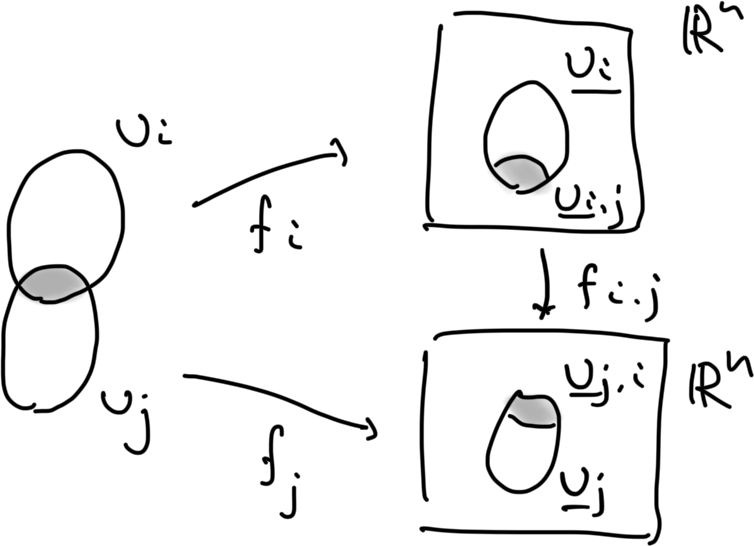
\includegraphics[scale=.3]{mfd.png} \]
\caption{Coordinate patches of a manifold \label{fig:coord-patch}}
\end{figure}

Suppose $U_i\cap U_j$ is nonempty. 
Let \begin{align}
\underline{U}_{i,j} &:= f_i(U_i\cap U_j) \subset \underline{U}_i,\\
\underline{U}_{j,i} &:= f_j(U_j\cap U_i)\subset \underline{U}_j.
\end{align}
Then we have the map \begin{equation}
f_{i,j} \colon \underline{U}_{i,j} \to \underline{U}_{j,i} 
\end{equation} defined by \begin{equation}
f_{i,j} := f_j \circ (f_i)^{-1} .
\end{equation}
This allows us to `paste together' $\underline{U}_i\subset \bR^n$ 
and $\underline{U}_j \subset \bR^n$
by identifying their subsets $\underline{U}_{i,j}$ and $\underline{U}_{j,i}$ using $f_{i,j}$.
%See Fig.~\ref{fig:pasting} for a drawing.


A smooth manifold is such that $f_{ij}$ are smooth;
a topological manifold is such that $f_{ij}$ are just required to be continuous.
A smooth manifold is automatically a topological manifold.
A bijective smooth map $f:M\to M'$ between two smooth manifolds $M$ and $M'$
is called a \emph{diffeomorphism};
a bijective continuous map $f:M\to M'$ between two topological manifolds $M$ and $M'$
is called a \emph{homeomorphism}.
In physics we typically consider smooth manifolds,
but I decided to include a bit of discussions about topological manifolds
as I thought the subtle concrete differences between smooth manifolds
and topological manifolds can be interesting to some of you.

\begin{theorem}
When a manifold $M$ is compact,
we can choose a finite number of coordinate patches $U_i$ to cover $M$.
\end{theorem}

Before going further, let us also introduce manifolds with boundaries:
\begin{definition}
  A \emph{manifold with boundary} is defined similarly,
  but we allow the neighborhood $\underline{U}$ to be in a half-space $\bR^{n-1}\times \bR_{\ge 0}$.
  The union of the inverse images of the boundary of 
  $\underline{U}\cap (\bR^{n-1} \times \{0\})$ 
  under $f$ is called \emph{the boundary of $M$}
  and is denoted by $\partial M$.
\end{definition}  

\begin{example}
  The half-space $\bR^{n-1}\times \bR_{\ge 0}$ is a manifold with boundary.
\end{example}

\begin{definition}
  A compact manifold without boundary is called a closed manifold.
\end{definition}


\subsection{Examples}
So far we only saw trivial examples.
We need better examples.

\subsubsection{Via equations}
A common way to construct manifolds is to take a subset of $\bR^n$ defined by a number of equations:
\begin{align}
f_1(x_1, x_2, \ldots, x_n) &= 0, \\
f_2(x_1, x_2, \ldots, x_n) &= 0, \\
&\vdots \\
f_m(x_1, x_2, \ldots, x_n) &= 0.
\end{align}
If the choice of $f_{1,2,\ldots,m}$ are sufficiently nice,
the set of points satisfying these equations is a manifold of dimension $n-m$.

A typical bad example is the subset of $\bR^2$ defined by $xy=0$: around $(x,y)=(0,0)$, two lines intersect, and therefore the neighborhood of $(0,0)$ is not of the right form.

\begin{example}
The $n$-dimensional sphere $S^n$ is defined by \begin{equation}
  x_1^2+x_2^2+\cdots+x_{n+1}^2=1.
\end{equation} 
\end{example}
Note that $S^n$ is embedded in $\bR^{n+1}$, but it is a manifold of dimension $n$.

\begin{example}
  The $n$-dimensional disk $D^n$ is defined by \begin{equation}
    x_1^2+x_2^2+\cdots+x_{n}^2\le 1.
  \end{equation} 
  This is a manifold with boundary, and the boundary is $S^{n-1}$.
  $D^n$ also called the $n$-dimensional ball and denoted by $B^n$.
\end{example}  

\begin{example}
$D^1$ is a segment $[-1,1]$ and its boundary $S^0$ consists of two points $\{-1,1\}$.
\end{example}

Calling two points, $S^0$, a 0-dimensional sphere sounds silly,
but it is just a name.
But this illustrates an important point:
you are not supposed to judge mathematical concepts by their names.
Rather, you are supposed to understand them by internalizing their definitions into your heart.

\begin{example}
  We can try considering points of constant Lorentz-invariant distance from the origin in $\bR^{d-1,1}$:
\begin{equation}
  x_1^2+x_2^2+\cdots+x_{d-1}^2-x_0^2=K ,
\end{equation}
where $K$ is a non-zero constant. 
This is a hyperboloid, and is a manifold of dimension $d-1$.
\end{example}
When $K>0$, it is connected; this is the hypersurface of spacelike-separated points 
of distance $\sqrt{|K|}$ from the origin
in the Minkowski spacetime.
When $K<0$, it consists of two components, one in the future $x_0>0$ and another in the past $x_0<0$.
They are the hypersurfaces of time-like separated points of temporal distance $\sqrt{|K|}$ from the origin.
When $K=0$, the equation above defines the lightcone, which is singular at the origin and is not a manifold.

We have various group manifolds, 
defined in a similar manner. 
Let $M_n(\bR)$ be the set of $n\times n$ real matrices.
\begin{example}
The orthogonal group $O(n)$ is defined by \begin{equation}
  O(n) = \{ M\in M_n(\bR) \mid M^T M = 1 \}.
\end{equation}
The special orthogonal group $SO(n)$ is defined by \begin{equation}
  SO(n) = \{ M\in O(n) \mid \det M = 1 \}.
\end{equation}
\end{example}

Similarly let $M_n(\bC)$ be the set of $n\times n$ complex matrices.
\begin{example}
The unitary group $U(n)$ is defined by \begin{equation}
  U(n) = \{ M\in M_n(\bC) \mid M^\dagger M = 1 \}.
\end{equation}
The special unitary group $SU(n)$ is defined by \begin{equation}
  SU(n) = \{ M\in U(n) \mid \det M = 1 \}.
\end{equation}
\end{example}

\begin{proposition}
$S^1=U(1)=SO(2)$.
\end{proposition}
This can be seen by parameterizing $S^1$ by $\theta \in [0,2\pi)$.
$U(1)$ is a one-by-one unitary matrix, i.e.~a complex number $z$ with $|z|=1$.
Therefore $z=e^{i\theta}$.
$SO(2)$ is a two-by-two orthogonal matrix with determinant $1$, which has the form \begin{equation}
  \begin{pmatrix}
    \cos\theta & -\sin\theta \\
    \sin\theta & \cos\theta
  \end{pmatrix}.
\end{equation}

\begin{proposition}
$S^3=SU(2)$.
\end{proposition}
This can be seen by noticing that any $SU(2)$ matrix has the form \begin{equation}
  \begin{pmatrix}
    z & -\overline w\\
    w & \overline z
  \end{pmatrix}
\end{equation} with $|z|^2+|w|^2=1$.
As $\bC^2\simeq \bR^4$, we see that this defines an $S^3$.
This fact can also be shown using quaternions $\bH$, 
introduced by Hamilton in 1843.
\begin{definition}
$\bH$ is a four-dimensional algebra over $\bR$ with a basis $1,i,j,k$ satisfying \begin{equation}
  i^2=j^2=k^2=-1, \quad
  ij=-ji=k, \quad
  jk=-kj=i, \quad
  ki=-ik=j.\label{eq:rel-of-H}
\end{equation}
\end{definition}

A general element is of the form $q=a+bi+cj+dk$ with $a,b,c,d\in \bR$.
The conjugate of $q=a+bi+cj+dk$ is $\bar q=a-bi-cj-dk$.
We can check that $\overline{q_1 q_2}=\bar q_2 \bar q_1$.

The norm of $q$ is $|q|^2=q\bar q=\bar q q=a^2+b^2+c^2+d^2$.
This is nonzero unless $q=0$.
This means that any nonzero element $q\neq 0$ has a multiplicative inverse $q^{-1}=\bar q/|q|^2$.
An algebra with this property is called a division algebra.
\begin{fact}
  The only finite-dimensional division algebras over $\bR$ are $\bR$, $\bC$, and $\bH$.
\end{fact}

Note also that $|q_1 q_2|^2=|q_1|^2 |q_2|^2$.
This means that the set $\{ q\in \bH \mid |q|=1 \}$ of unit quaternions forms a group.
As $\bH\simeq \bR^4$, this is a three-dimensional sphere $S^3$.
Considering $\bH\simeq \bC^2$, we can convince ourselves that this is also $SU(2)$.
More generally:
\begin{example}
  The unitary symplectic group $Sp(n)$ is defined by \begin{equation}
    Sp(n) = \{ M\in M_{n}(\bH) \mid M^\dagger M = 1 \}.
  \end{equation}
\end{example}
In particular, $Sp(1)=SU(2)=S^3$.
Note there is no distinct `special unitary symplectic group'.

To explain $Sp(m)$ a bit more geometrically, consider $\bH^n$
as the space of column vectors of quaternions. 
We consider `linear' maps  $M:\bH^n\to \bH^n$ in the sense that
\begin{equation}
M (vq) = (Mv) q, \qquad v\in \bH^n,\ q\in \bH.
\end{equation} 
(Note that the placement of $q$ on the right is important, 
as the multiplication is non-commutative in $\bH$.)
Denote the basis vectors by $e_1,e_2,\ldots,e_n$.
Then such an $M$ is specified by \begin{equation}
M e_i = \sum_j M_{ij} e_j.
\end{equation}
The condition $M^\dagger M=1$ is the condition that it preserves the norm $|v|$ of $v\in \bH^n$
defined by \begin{equation}
  |v|^2 := \sum_i |v_i|^2.
\end{equation}

\begin{fact}
  The only cases when $S^n$ is a group are $S^0=O(1)=\{1,-1\}$, $S^1=SO(2)=U(1)$
  and $S^3=SU(2)=Sp(1)$.
\end{fact}
  
\subsubsection{Time reversal and $\bR$, $\bC$, $\bH$}

Let me make a side remark concerning the natural role of $\bH$ in quantum mechanics.
Let's consider a quantum mechanical system with finite-dimensional Hilbert space $\cH$.
The time reversal operator $\sT$ is anti-unitary, in that 
\begin{equation}
  \sT z = \overline z \sT.
\end{equation}
Assuming that $\sT^2=c$ with a constant $c$, let's show $c=\pm1$. We evaluate $\sT^3$ in two orders:
\begin{equation}
\sT(\sT^2)= \sT c = \overline{c}\sT,\qquad
(\sT^2)\sT = c\sT.
\end{equation} Therefore $c=\overline{c}$. As the unitarity of $\sT^2$ requires $|c|=1$,
 we find $c=\pm 1$.

 \paragraph{The case $c=+1$:}
 This case, any vector $v\in \cH$ can be decomposed into its real and imaginary parts:
  \begin{equation}
    v = v_\text{re} + v_\text{im} i 
  \end{equation}
  where
  \begin{equation}
    v_\text{re}:= \frac{1+\sT}{2} v, \quad v_\text{im}:=\frac{1-\sT}{2i}v .
  \end{equation}
  Note that $T v_\text{re}= v_\text{re}$ and $T v_\text{im}=v_\text{im}$.
So, the $T$-invariant part of $\cH$ is a real vector space.
Denoting it by $\cH_\bR$, we see that if $\cH_\bR=\bR^n$, $\cH=\bC^n$.
Unitary matrices acting on $\cH$ commuting with $\sT$
are orthogonal matrices acting on $\cH_\bR$.
So, time-reversal-invariant unitary operators on $\cH$ 
form the group $O(n)$.

\paragraph{The case $c=-1$:}
In this case, we note that $i$, $j:=\sT$, $k:=i \sT$ satisfy 
the defining relation \eqref{eq:rel-of-H} of $\bH$.
(More precisely, we can equip the space $\cH$ of quantum states
with an action of $\bH$ from the right, via $vi := iv$ and $vj:=\sT v$.)

Therefore, $\cH= \bH^m$ for some $m$. When $\cH=\bC^n$, this forces $n=2m$ to be even.
This is known as Kramers degeneracy.

A unitary operator commuting with $\sT$
is a norm-preserving map on $\bH^m$ which commutes with the quaternion action from the right.
Therefore it belongs to $Sp(m)$.

\paragraph{Summary:}
$U(n)$, $SO(n)$, and $Sp(n/2)$ are the groups of norm-preserving linear operators
on a quantum system $\cH=\bC^n$ with $n$ states with the following conditions:
\begin{itemize}
\item $U(n)$: no time reversal,
\item $SO(n)$: time reversal with $\sT^2=+1$,
\item $Sp(n/2)$: time reversal with $\sT^2=-1$; $n$ is forced to be even.
\end{itemize}


\subsubsection{Via combinations}

Let's come back to the examples of manifolds.

\begin{notation}
 Given two manifolds $M$ and $N$ of dimensions $m$ and $n$,
 we write its product as $M\times N$.
It is a manifold of dimension $m+n$.
\end{notation}

\begin{notation}
Given two manifolds $M$ and $N$ of the same dimension $n$,
we write its disjoint union as $M\sqcup N$.
It is a manifold of dimension $n$.
\end{notation}

Note that $S^1\times S^1$ is two-dimensional and the surface of a donut,
while $S^1\sqcup S^1$ consists of two circles and is one-dimensional.

\begin{example}
  The $n$-dimensional torus is \begin{equation}
    T^n = \underbrace{S^1\times S^1\times \cdots \times S^1}_\text{ $n$ times}.
  \end{equation}
\end{example}

\begin{example}
$S^1\times [-1,1]$ is a cylinder. Its boundary is $S^1\sqcup S^1$.
\end{example}

Another construction is the following:
\begin{notation}
  Given two connected manifolds $M$, $N$ of dimension $n$,
  pick points $p\in M$ and $q\in N$.
  remove small open balls $B^n(p)$ and $B^n(q)$ from $M$ and $N$, and
  paste the common $S^{n-1}$ boundary.
  The result is the connected sum $M\# N$.
\end{notation}

For example, the connected sum 
\begin{equation}
  \underbrace{T^2 \# T^2 \# \cdots \# T^2}_\text{$g$ copies}
\end{equation}
is the surface of a multi-donut (whatever that is).
More professionally, it is called a genus-$g$ surface.
$S^2$ is defined to have genus 0.

\begin{fact}
Any two-dimensional compact connected oriented manifold is $S^2$ or 
the surface of a multi-donut with $g$ holes.
\end{fact}

\subsubsection{Via quotients}

Another method to define manifolds is to 
take the quotient of a manifold by a group action. 
Let us explain it more fully.
\begin{definition}
A \emph{group action} of a group $G$ on a manifold $M$ is a map \begin{equation}
  G\times M \to M, \quad (g, p) \mapsto g p
\end{equation} such that \begin{equation}
  e p = p, \quad (gh) p = g (h p)
\end{equation} for all $g,h\in G$ and $p\in M$.
Here $e$ is the identity in $G$.
\end{definition}
We often want the action to be smooth or at least continuous,
depending on the context.

\begin{definition}
Let $p\sim q$ if there is a $g\in G$ such that $g p = q$.
The quotient space $M/G$ is the set $M/\sim$ of equivalence classes 
under this relation.
\end{definition}

$M/G$ is not always a manifold.
For example, consider $\bR^3$ with the action of $\bZ_2$ generated by 
\begin{equation}
(x,y,z) \mapsto (-x,-y,-z).
\end{equation}
The origin is singular, and the quotient space $\bR^3/\bZ_2$ is not a manifold.
(It still belongs to a larger class of spaces called \emph{orbifolds}.)
It is complicated to state the conditions under which $M/G$ is a manifold,
so we will not do so in this lecture series.

We now define the real, complex and quaternionic projective spaces $\RP^n$, $\CP^n$ and $\HP^n$ uniformly.
\begin{example}
  For $\bK=\bR,\bC,\bH$, 
  consider the action of $\bK\setminus \{0\}$ on
  $\bK^{n+1}\setminus\{0\}$ by scalar multiplication.
  The projective space $\KP^n$ is then defined as
  \begin{equation}
    \KP^n = (\bK^{n+1}\setminus\{0\})/(\bK\setminus\{0\}).
  \end{equation}
  These are of dimension $n$, $2n$, and $4n$ respectively.
\end{example}
More directly, we consider elements 
\begin{equation}
(x_1,x_2,\ldots,x_{n+1})\in \bK^{n+1}
\end{equation} such that not all of $x_i$ is zero.
Then we make the identification \begin{equation}
  (x_1,x_2,\ldots,x_{n+1}) \sim  ( x_0, x_1, \ldots,  x_n)c \label{eq:proj-ident}
\end{equation} for nonzero $c\in \bK$.
A point on $\KP^n$ is often denoted by $[x_1:x_2:\cdots:x_{n+1}]$.

Before proceeding, we note that $\CP^n$ parameterize physically-distinct pure states 
in an $(n+1)$-dimensional Hilbert space.
Indeed, two nonzero ket vectors $\ket{\psi}$ and $\ket{\psi'}$ represent the same physical state
when there is a complex number $c$ such that $\ket{\psi'}=c\ket{\psi}$.
This is exactly the condition \eqref{eq:proj-ident}.

It is instructive to give explicit coordinate patches.
Let $U_i$ be the points on $\CP^n$ with $x_i\neq 0$.
Note that when $x_i\neq 0$, we have \begin{equation}
  (x_1,x_2,\ldots,x_{n+1}) \sim (x_1/x_i, x_2/x_i, \ldots, x_i/x_i=1, \ldots, x_{n+1}/x_i).
\end{equation} 
In other words, we can introduce coordinates on $U_i$ by defining  $y_k:=x_k/x_i$ for $k\neq i$;
equivalently, we constructed a map $f_i: U_i \to \underline{U}_i \simeq \bK^n$.

Let us consider another patch $U_j$ containing points with $x_j\neq 0$. 
We introduce coordinates $z_k:=x_k/x_j$ for $k\neq j$;
this gives the map $f_j: U_j \to \underline{U}_j\simeq \bK^n$.

$U_i$ and $U_j$ overlap when $x_i\neq 0$ and $x_j\neq 0$.
We then need to find the coordinate transformation 
between $f_i(U_i \cap U_j )\subset \underline{U}_i$
and $f_j(U_i \cap U_j) \subset \underline{U}_j$, realizing the identification of
\begin{equation}
  (y_1,y_2,\ldots,y_{n+1}) \quad \text{with $y_i=1$, $y_j\neq 0$}
\end{equation} and 
\begin{equation}
  (z_1,z_2,\ldots,z_{n+1}) \quad \text{with $z_j=1$, $z_i\neq 0$}.
\end{equation}
This is done by setting $z_k = y_k / y_j$, where $y_i$ was defined to be $=1$.

From this description we see \begin{equation}
\RP^1=S^1,\quad
\CP^1=S^2,\quad
\HP^1=S^4.
\end{equation}
Indeed, in this case we have two patches \begin{equation}
  U_1 = \{ [1:y] \mid y\in \bK \}, \quad U_2 = \{ [z:1] \mid z\in \bK \}.
\end{equation} where $z=y^{-1}$ in the overlap $U_1\cap U_2$.
$U_1$ is the northern hemisphere,
$U_2$ is the southern hemisphere,
and they are patched to form a sphere in the appropriate dimensions.

Another way to look at $\KP^n$ is the following. 
To pick a representative under the identification \eqref{eq:proj-ident},
we first fix $\sum_i |x_i|^2 =1$.
As $\bK^{n+1}=\bR^{p(n+1)}$ where $p=1,2,4$ for $\bK=\bR,\bC,\bH$,
we have $S^n$, $S^{2n+1}$, $S^{4n+3}$ at this point.

The identification \eqref{eq:proj-ident} still acts within this sphere
if $|c|=1$. 
Depending on $\bK=\bR,\bC,\bH$, the group of such $c$ is $O(1)=\{\pm1\}=S^0$, $U(1)=S^1$, $Sp(1)=SU(2)=S^3$, respectively.
Therefore, we have \begin{equation}
\RP^n=S^n/O(1), \quad \CP^n=S^{2n+1}/U(1), \quad \HP^n=S^{4n+3}/Sp(1).
\end{equation}



\subsubsection{Non-orientable surfaces}

\begin{example}
  Consider $S^1\times [-1,1]$, parameterized by $\theta\sim \theta+2\pi$ and $x\in [-1,1]$.
  We can consider the $\bZ_2$ action $(\theta,x)\mapsto (\theta+\pi,-x)$.
  The quotient space is called the M\"obius strip.
  This is non-orientable, and the boundary is a single circle $S^1$.
\end{example}

As a non-orientable closed manifold, 
we have $\RP^2$ we introduced above. To see this, recall $\RP^2=S^2/\bZ_2$,
where the $\bZ_2$ action identifies the antipodal points. 
Any point on the southern hemisphere is identified with some point on the northern hemisphere.
Then $\RP^2$ can be identified with the northern hemisphere
whose boundary, i.e.~the equator, has an extra identification $\theta \sim \theta+\pi$.

Let us have a closer look at the neighborhood of the equator.
We can parameterize it by the longitude $\theta$ together with the latitude $\phi\in (-\epsilon,\epsilon)$.
The antipodal identification is $(\theta,\phi)\sim (\theta+\pi,-\phi)$.
This is the same as the M\"obius strip, which is non-orientable.
In string theory, this local structure around the equator is called a crosscap (叉帽).
Another way to say this is that $\RP^2$ is obtained by pasting a northern hemisphere (i.e.~a disk)
to a M\"obius strip along the boundary.

Another non-orientable surface can be constructed by the quotient.
\begin{example}
Consider $T^2$ parameterized by $\theta$ and $\phi$
with the identification $\theta\sim \theta+2\pi$ and $\phi \sim \phi+2\pi$,
and take a further identification as above: $(\theta,\phi)\sim (\theta+\pi,-\phi)$.
The result is known as the Klein bottle.
\end{example}
Locally around $\phi=0$ and $\phi=\pi$, we have two M\"obius strips.
So the resulting surface is obtained by pasting two M\"obius strips along the boundary.
Equivalently, it is obtained by taking the connected sum $\RP^2\#\RP^2$.

We can consider many other non-orientable surfaces by taking a repeated connected sum:
\begin{equation}
  \underbrace{\RP^2\#\RP^2\#\cdots\#\RP^2}_\text{$h$ copies}
  \#
  \underbrace{T^2\# T^2 \#\cdots\# T^2}_\text{$g$ copies}
\end{equation}
where we take $h>0$ and $g\ge 0$.
In fact, many of them are actually homeomorphic to each other.
\begin{fact}
Any compact connected non-orientable 2d surface is homeomorphic to
\begin{equation}
\RP^2 \# \underbrace{T^2\# T^2 \#\cdots\# T^2}_\text{$g$ copies}
\end{equation}
or the Klein bottle $\RP^2\#\RP^2$.
\end{fact}
It is a fun exercise to show that $\RP^2 \# \RP^2 \# \RP^2$ is homeomorphic to $\RP^2 \# T^2$.

\subsubsection{Some other fun manifolds}


\paragraph{The de-singularization of $\bC^2/\bZ_2$:}
Let's consider $\bC^2$ parameterized by $(z,w)$,
and consider the $\bZ_2$ action $(z,w)\mapsto (-z,-w)$.
The quotient space $\bC^2/\bZ_2$ is singular at the origin.
We can parameterize the same space in a different way:
Let $(s,t,u):=(z^2, z w, w^2)$.
Then the $\bZ_2$ action is trivial on $(s,t,u)$, but we have the relation $su=t^2$.
From $(s,t,u)$ satisfying $su=t^2$, we can uniquely reconstruct $(z,w)\simeq -(z,w)$.
So $\bC^2/\bZ_2$ can be identified with the subspace \begin{equation}
X=\{ (s,t,u)\in \bC^3 \mid su=t^2 \}.
\end{equation}
We can desingularize $X=\bC^2/\bZ_2$ it in the following way.

We add the variables $(x_1,x_2)\in \bC^2\setminus \{0\}$, with the identification 
$(x_1,x_2)\sim a(x_1,x_2)$ for $a\in \bC\setminus \{0\}$,
i.e.~we introduce $\CP^1\simeq S^2$.
Recall that its points are denoted by $[x_1:x_2]$.
We now add a further constraint \begin{equation}
(z,w) = c(x_1,x_2) \quad \text{for some $c\in \bC$},
\end{equation} or equivalently \begin{equation}
  (s,t,u)= c'(x_1^2, x_1 x_2, x_2^2) \quad \text{for some $c'\in \bC$}. \label{eq:blowup}
\end{equation}

Denote the total space by $\tilde X$: 
it is a subspace of $\bC^3\times \CP^1$ 
parameterized by 
$(s,t,u,[x_1:x_2])$ 
under the constraints $su=t^2$ and \eqref{eq:blowup}.
This space comes with two projections maps, $\pi_1:\tilde X\to X=\bC^2/\bZ_2$ 
given by taking $(s,t,u)$
and $\pi_2:X\to \CP^1$ given by taking $[x_1:x_2]$.

Note that $\pi_1$ is one-to-one except at the origin, $(z,w)=(0,0)$.
It is because the relation \eqref{eq:blowup} uniquely determines $[x_1:x_2]=[z:w]$.
At the origin, $(z,w)=(0,0)$, the inverse image is the entirety of $\CP^1$. 
So, $\tilde X$ can be thought of inserting  $\CP^1$ at the origin of $X=\bC^2/\bZ_2$.

$\tilde X$ is actually a smooth manifold.
To see this, we consider the second projection $\pi_2: \tilde X\to \CP^1$.
Given a point $[x_1:x_2]\in \CP^1$,
the inverse image of $\pi_2$ is simply $c'(x_1^2, x_1 x_2, x_2^2)\in \bC$
for $c'\in \bC$. 
So it is isomorphic to a copy of $\bC$.
So $\tilde X$ can be visualized as a copy of $\bC$ attached smoothly at each point of $\CP^1$,
and is a smooth manifold.

\paragraph{A K3 manifold:}

The manifold $\tilde X$ introduced above was non-compact. 
It can be used to construct a rather important compact manifold of dimension 4.
We start from $T^4$ parameterized by $\theta_i\in \bR$ with the identification $\theta_i\sim \theta_i+2\pi$, for $i=1,2,3,4$.
We consider the $\bZ_2$ action given by \begin{equation}
  (\theta_1,\theta_2,\theta_3,\theta_4) \mapsto -(\theta_1,\theta_2,\theta_3,\theta_4).
\end{equation}
Note that $theta \sim -\theta$ under the identification $\theta\sim \theta+2\pi$ when $\theta=0,\pi$.
The quotient space $T^4/\bZ_2$ is therefore singular at $2^4=16$ points
when $\theta_i = 0,\pi$ for $i=1,2,3,4$.
Around each point, it locally has the form $\bR^4/\bZ_2 = \bC^2/\bZ_2$ studied above.
Then, we can insert 16 copies of $\CP^1$ at these 16 points to desingularize the space.
The result is a smooth compact manifold of dimension 4, 
and is an example of a class of manifold called K3.\footnote{%
The name K3 was introduced by the mathematician A. Weil, after the three mathematicians 
Kummer, K\"ahler, and Kodaira who studied it, and also the mountain K2 in the Himalayas.
The construction given here is due to Kummer.
}

\subsection{Some fun facts about manifolds}

\subsubsection{Smooth vs.~topological manifolds}
Consider the following equation in $\bC^5$:
\begin{equation}
z_1^2+z_2^2+z_3^2+z_4^3+z_5^{6k-1}=0.  
\end{equation} Except at the origin, it is a smooth manifold of complex dimension 4, 
i.e.~of real dimension 8.
We can take the intersection with the unit sphere $S^9=\{\sum|z_i|^2=1\}$ in $\bC^5$.
This results in a smooth compact manifold $M_k$ of dimension 7.
It is known that $M_k$ are all homeomorphic to the standard $S^7$,
but they are not diffeomorphic to it unless $k$ is a multiple of $28$.
In fact, there are exactly 28 ways to make $S^7$ into a smooth manifold,
and the construction above exhausts them.
This goes back to Milnor in 1956; a very readable account is given e.g.~in \cite{MeerThesis}.
These manifolds are called exotic spheres, 
but they are not very exotic, as the explicit equation above shows!

There are also cases where a topological manifold does not admit any smooth structure.
That there are such manifolds in four dimensions was realized by Freedman \cite{Freedman} in 1982.
An example is called as the $E_8$ manifold.
Again the construction with coordinate patches with continuous maps between them is explicit;
what was difficult was to show that there cannot be any smooth structure. 
Next year in 1983, Donaldson \cite{Donaldson} 
introduced a new method to study smooth four-dimensional manifolds
using gauge theory, with many spectacular results.
One result which was soon found that $\bR^4$ also has a smooth structure 
which is not diffeomorphic to the standard one.
(For example, in one of such exotic smooth structures, 
any smoothly embedded $S^3$ in it resides in a compact region around the origin.
So, there can't be an arbitrarily large $S^3$ in it.)

\subsubsection{Triangulation of manifolds}
Two-dimensional surfaces can be triangulated. 
We can ask the same question in higher dimensions,
where we replace triangles by simplices. (A simplex in dimension $n$ has $n+1$ vertices, etc.)
Can manifolds be triangulated?
It is known that smooth manifolds can be triangulated. 
How about topological manifolds?

Well, the four-dimensional $E_8$ manifold above cannot be triangulated.
The situation in dimensions more than five was more subtle.
It was shown by Matumoto \cite{Matumoto} in 1978 and Galewski-Stern \cite{GalewskiStern} in 1980 that,
all topological manifolds of dimension $n\ge 5$ can be triangulated
\emph{if} there exists a \emph{three}-manifold satisfying certain properties.
If no such three-dimensional manifold exists,
then for every dimension $n\ge 5$ there are topological manifolds which cannot be triangulated.
Non-existence of such a three-manifold was finally proved by Manolescu \cite{Manolescu} in 2013.
This work used a mathematical version of Seiberg-Witten theory,
which originated in the study of supersymmetric gauge theory 
in theoretical physics by Seiberg and Witten in the mid-1990s,
who showed how confinement happens in a supersymmetric version of QCD.
This mathematical Seiberg-Witten theory 
can be considered as an easier version of Donaldson's theory referred to above,
and has been developed vigorously by mathematicians since its introduction.


\subsubsection{Some comments}
So we have hierarchy of structures on manifolds: \begin{multline}
  \{\text{topological manifolds}\}
  \supset
  \{\text{triangulated manifolds}\} \\
  \supset
  \{\text{PL manifolds}\}
  \supset
  \{\text{smooth manifolds}\}
\end{multline}
where I added another stage, known as piecewise-linear (PL) manifolds,
which can be found more often discussed in the math literature 
than triangulated manifolds.\footnote{%
PL manifolds are triangulated manifolds such that
for each vertex $v$, the link of $v$ (the polyhedron formed by 
simplices immediately surrounding $v$) is piece-wise-linear isomorphic to $S^{n-1}$.
}
There are various differences at each stage, as we have seen above.

Why do we/I care about these things?
I don't really know.  But let me give some excuses.
\begin{itemize}
  \item Firstly, it's simply interesting, at least to me.
\item Secondly, it is particularly interesting that gauge-theoretic (and therefore physics-inspired)
methods were used to study these issues.
\item Thirdly, I found the following difference between hep-th and cond-mat people:
In hep-th, we often consider smooth manifolds as given (as in general relativity),
whereas in cond-mat, manifolds only appear as long-range approximation of a more fundamental
lattice structure. 
In theoretical condensed-matter physics, a general manifold is often studied
assuming that it is equipped with a triangulation. 
Therefore, I think that it might be of some use to be aware of the distinction between
these two approaches to manifolds.
For example, it seems possible to write down
the Hamiltonian of a strange symmetry-protected topological phase
which is defined on triangulated manifolds such that
it detects non-smooth but triangulable manifolds, 
although in a rather high dimensionality meaningless in our actual world.
\end{itemize}

\section{Fiber bundles}

\subsection{Definition}

\begin{definition}
fiber bundles
\end{definition}

\begin{example}
M\"obius strip
\end{example}



\subsection{Quotients as bundles}

\begin{example}
general quotients
\end{example}

\begin{definition}
principal G-bundles = free quotients
\end{definition}

\begin{example}
projective spaces
\end{example}

\begin{example}
$S^1\to S^3\to S^2$ as Bloch sphere
\end{example}

\begin{example}
$S^3\to S^7\to S^4$
\end{example}

\begin{fact}
Hopf fibrations
\end{fact}

\begin{definition}
homogeneous spaces and orbit spaces
\end{definition}

\begin{example}
$S^1\to S^3\to S^2$ as symmetry breaking by a vev
\end{example}

\begin{example}
superfluid Helium-3 A-phase 
\end{example}

\subsection{Vector bundles}


\begin{definition}
vector bundles
\end{definition}

\begin{definition}
line bundles
\end{definition}

\begin{definition}
unit sphere bundle
\end{definition}

\begin{definition}
subbundle
\end{definition}

\begin{example}
$S^1\to S^3\to S^2$
as lowest energy states of a parameterized Hamiltonoian
\end{example}

operations: 
direct sum,
dual,
complex conjugate,
tensor product,
(anti)-symmetric tensor powers, 
projectivization, etc.

\begin{example}
bundle of Hilbert spaces and bundle of density matrices.
\end{example}



\subsection{Examples: tangent and related bundles}

\begin{example}
tangent bundle
\end{example}

\begin{example}
cotangent bundle
\end{example}

\begin{example}
differential forms
\end{example}

\begin{example}
metric
\end{example}


\begin{definition}
structure group of a bundle
\end{definition}

\begin{definition}
lifts / reduction of structure groups
\end{definition}


\begin{example}
reduction from $GL$ to $O$
\end{example}

\begin{definition}
reduction from $O$ to $SO$
\end{definition}

\begin{fact}
spin groups in general dimensions.
\end{fact}

\begin{fact}
spin groups in dimension 3 and 4.
\end{fact}

\begin{definition}
associated vector bundle
\end{definition}

\begin{definition}
spin structure and the spinor bundle
\end{definition}

\begin{fact}
oriented three-dimensional manifolds is always spin.
\end{fact}

\begin{fact}
$\CP^2$ is not spin.
\end{fact}

\subsection{Gauge fields and $G$-bundles}

\begin{definition}
connection = gauge field
\end{definition}

\begin{definition}
covariant derivative
\end{definition}

\begin{example}
Schr\"odinger eq.~in the presence of magnetic field
\end{example}

\begin{example}
$S^1\to S^3\to S^2$ as Dirac monopole
\end{example}

\begin{example}
affine connection, spin connection
\end{example}
 
\begin{example}
Gauge fields of the Standard Model
\end{example}

\begin{example}
Matter content of the Standard Model
\end{example}

\subsection{Pin and spin groups in general dimensions}




\section{Basic homotopy theory}
\label{sec:basic-homotopy}

\subsection{Definitions and basic properties}


\begin{definition}
homotopy class of maps
\end{definition}

\begin{definition}
homotopy equivalence
\end{definition}

\begin{definition}
homotopy groups of spaces
\end{definition}

\begin{theorem}
$\pi_{n}(X)$ for $n\ge 2$ is Abelian.
\end{theorem}

\begin{theorem}
$\pi_n(X\times Y)$.
\end{theorem}

\begin{example}
$\pi_1(\Sigma_g)$
\end{example}

\begin{example}
$\pi_1(S^n/\Gamma)$
\end{example}


\subsection{Facts on $\pi_n(S^m)$}

\begin{theorem}
$\pi_n(S^m) =0$ if $n<m$
\end{theorem}

\begin{theorem}
$\pi_n(S^n) =\bZ_n$
\end{theorem}

\begin{theorem}
$\pi_3(S^2)=\bZ$.
\end{theorem}

\begin{theorem}
$\pi_{2n-1}(S^n)$ contains a  $\bZ$ summand.
Otherwise they are all torsion.
\end{theorem}

\begin{theorem}
$\pi_4(S^3)=\bZ_2$
\end{theorem}

\begin{definition}
suspension homomorphism
\end{definition}

\begin{theorem}
Freudenthal suspension theorem
\end{theorem}

\begin{definition}
Stable homotopy groups of spheres
\end{definition}

\begin{fact}
Stable homotopy groups of spheres
\end{fact}

`Mahowald uncertainty principle'

\subsection{Fiber bundles and homotopy groups}

\begin{definition}
long exact sequence of groups
\end{definition}

\begin{theorem}
long exact sequence of homotopy groups
\end{theorem}

\begin{example}
$\pi_1(S^n/\Gamma)$ again
\end{example}

\begin{example}
$\pi_3(S^2)$ via Hopf fibration
\end{example}

\begin{example}
$\pi_5(SU(2))\to \pi_5(SU(3)) \to \pi_5(S^5) \to \pi_4(SU(2))$ 
\end{example}

\subsection{Topological solitons and homotopy groups}

\subsubsection{Those associated to the space of order paremeters}

With codimension $d$ and the target space $X$, 
we have solitons in $\pi_d(X)$.

\begin{example}
Skyrmion
\end{example}

\begin{example}
Hopfion
\end{example}


\subsubsection{Those associated to symmetry breaking}

With codimension $d$ and the symmetry breaking pattern $H\subset G$,
we have solitons in $\pi_{d-1}(G/H)$.

(We can also have $\pi_d(G/H)$ as above, since $G/H$ is the space of order parameters. ???)

\begin{example}
Abrikosov/Nielsen-Olsen vortex
\end{example}

\begin{example}
't Hooft-Polyakov monopole 
\end{example}

\begin{example}
Superfluid Helium 3 A-phase
\end{example}

\begin{example}
`Instanton particle'
\end{example}

\section{Differential forms and de Rham cohomology}


\section{Cellular cohomology}

\section{Characteristic classes}

\section{Classifying spaces}

\section{Chern-Simons terms and bordism groups}

\section{K-theory}

\section{Atiyah-Singer index theorem}

\section{Anomalies}

\section{Computing \texorpdfstring{$\pi_4(S^3)$}{pi4(S3)}}

\bibliographystyle{ytamsalpha}
%\baselineskip=.85\baselineskip%\let\ttfamily\relax
%\let\bbb\bibitem\def\bibitem{\itemsep1pt\bbb}
\bibliography{ref}

\end{document}
